% !TeX source = ../main.tex

\chapter[A priori error estimates (Lax-Milgram case)]{A priori error estimates (Lax-Milgram case)}

\section{Triangulation of the domain $\Omega$}
In FEM (Finite Element Methods) we discretize the domain $\Omega$ in \emph{simple subdomains} (like triangles for example) where it's easy to define polynomials. Formally speaking we partition $\Omega$
\begin{equation*}
\Omega = \Bigl(\bigcup_{m=1}^M T_m \Bigr)
\end{equation*}
where 
\begin{equation}
T_i \cap T_j = \begin{cases}\emptyset \\ \text{vertex} \\ \text{boundary face}.\end{cases}
\end{equation}
We call this partition \emph{triangulation}. We emphasize that triangulation is just an historical term: we can have triangulations composed of different shapes.

Generally speaking the domain $\Omega$ might be a manifold so it might be needed to have some kind of family of maps (an atlas) that connects a "generic standard" element (we will call it reference triangle) of the triangulation to the true elements of the partitioning of $\Omega$. 

\section{Scaling argument for Sobolev norms}

%%%%%
% Lecture of 20 of March
%%%%%
\begin{figure}[!ht]
\centering
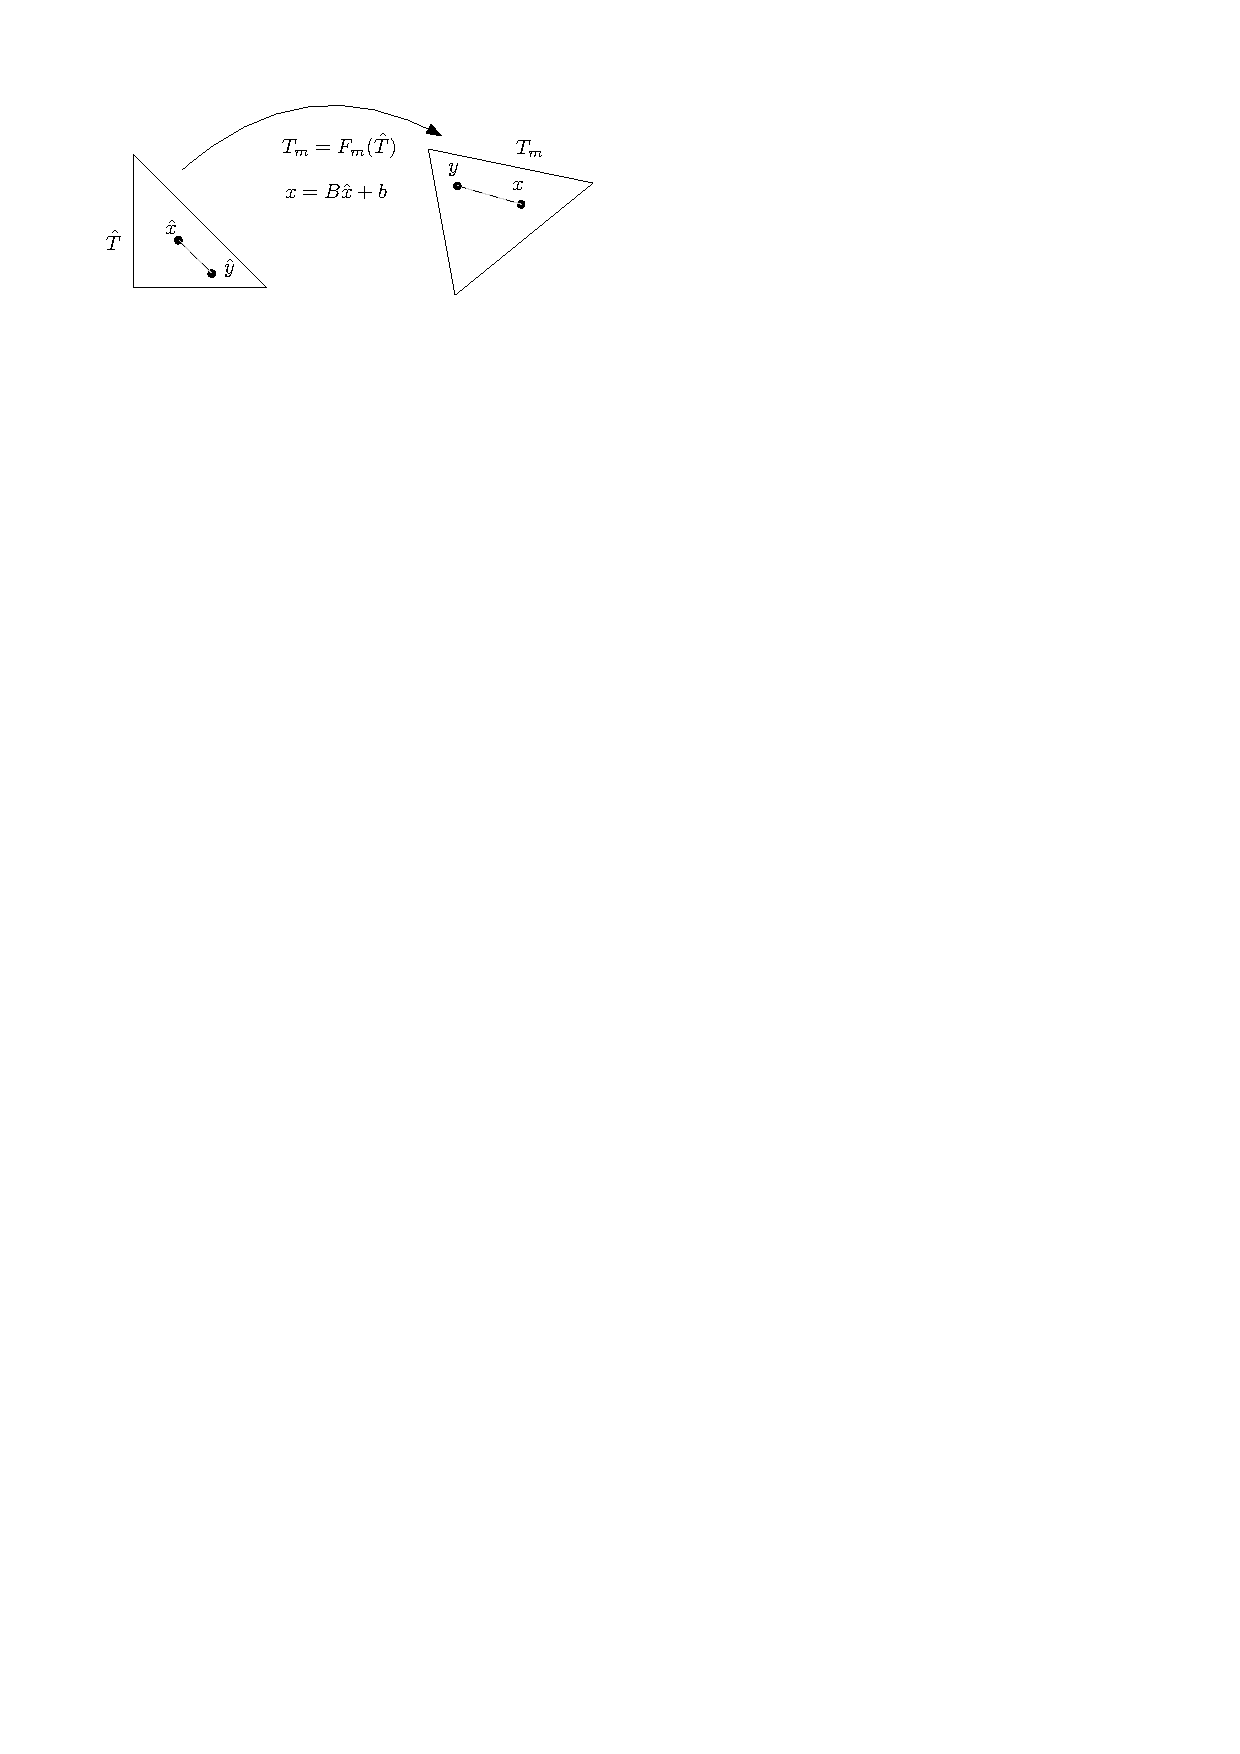
\includegraphics{affine_mapping}
\caption{A triangle $T_m$ and its reference triangle $\hat{T}$. The affine mapping $F_m$ maps $\hat{T}$ to $T_m$.}
\label{fig:affine_mapping}
\end{figure}

Consider an affine mapping from a reference triangle $\hat T$, to a generic triangle $T_m$ (Figure~\ref{fig:affine_mapping}):
\begin{align}
F_m: &\hat{T} \to T_m \\
&\hat{x} \mapsto x = B \hat{x} + b.
\end{align}
We would like to analyze how Sobolev norms change under the action of $F_m$. Recall the the definition of the Sobolev norm in $W^{k,p}$:
\[
\norm{v}^p_{k,p,\Omega} = \sum_{\abs{\alpha} \le k} \norm{D^\alpha v}^p_{L^p(\Omega)},
\]
with the corresponding seminorm:
\[
\abs{v}^p_{k,p,\Omega} = \sum_{\abs{\alpha} = k} \norm{D^\alpha v}^p_{L^p(\Omega)}.
\]

Let
\[
\rho_m := \sup_{\tilde{B} \subset T_m} \diam(\tilde{B}), \quad h_m := \inf_{T_m \subset \tilde{B}} \diam(\tilde{B}),
\]
and similarly for the reference triangle $\hat{T}$:
\[
\hat{\rho} := \sup_{\tilde{B} \subset \hat{T}} \diam(\tilde{B}), \quad \hat{h} := \inf_{\hat{T} \subset \tilde{B}} \diam(\tilde{B}),
\]
where $\tilde{B}$ denotes a ball in the right space (see Figure~\ref{fig:scaling}).


\begin{figure}[!ht]
\centering
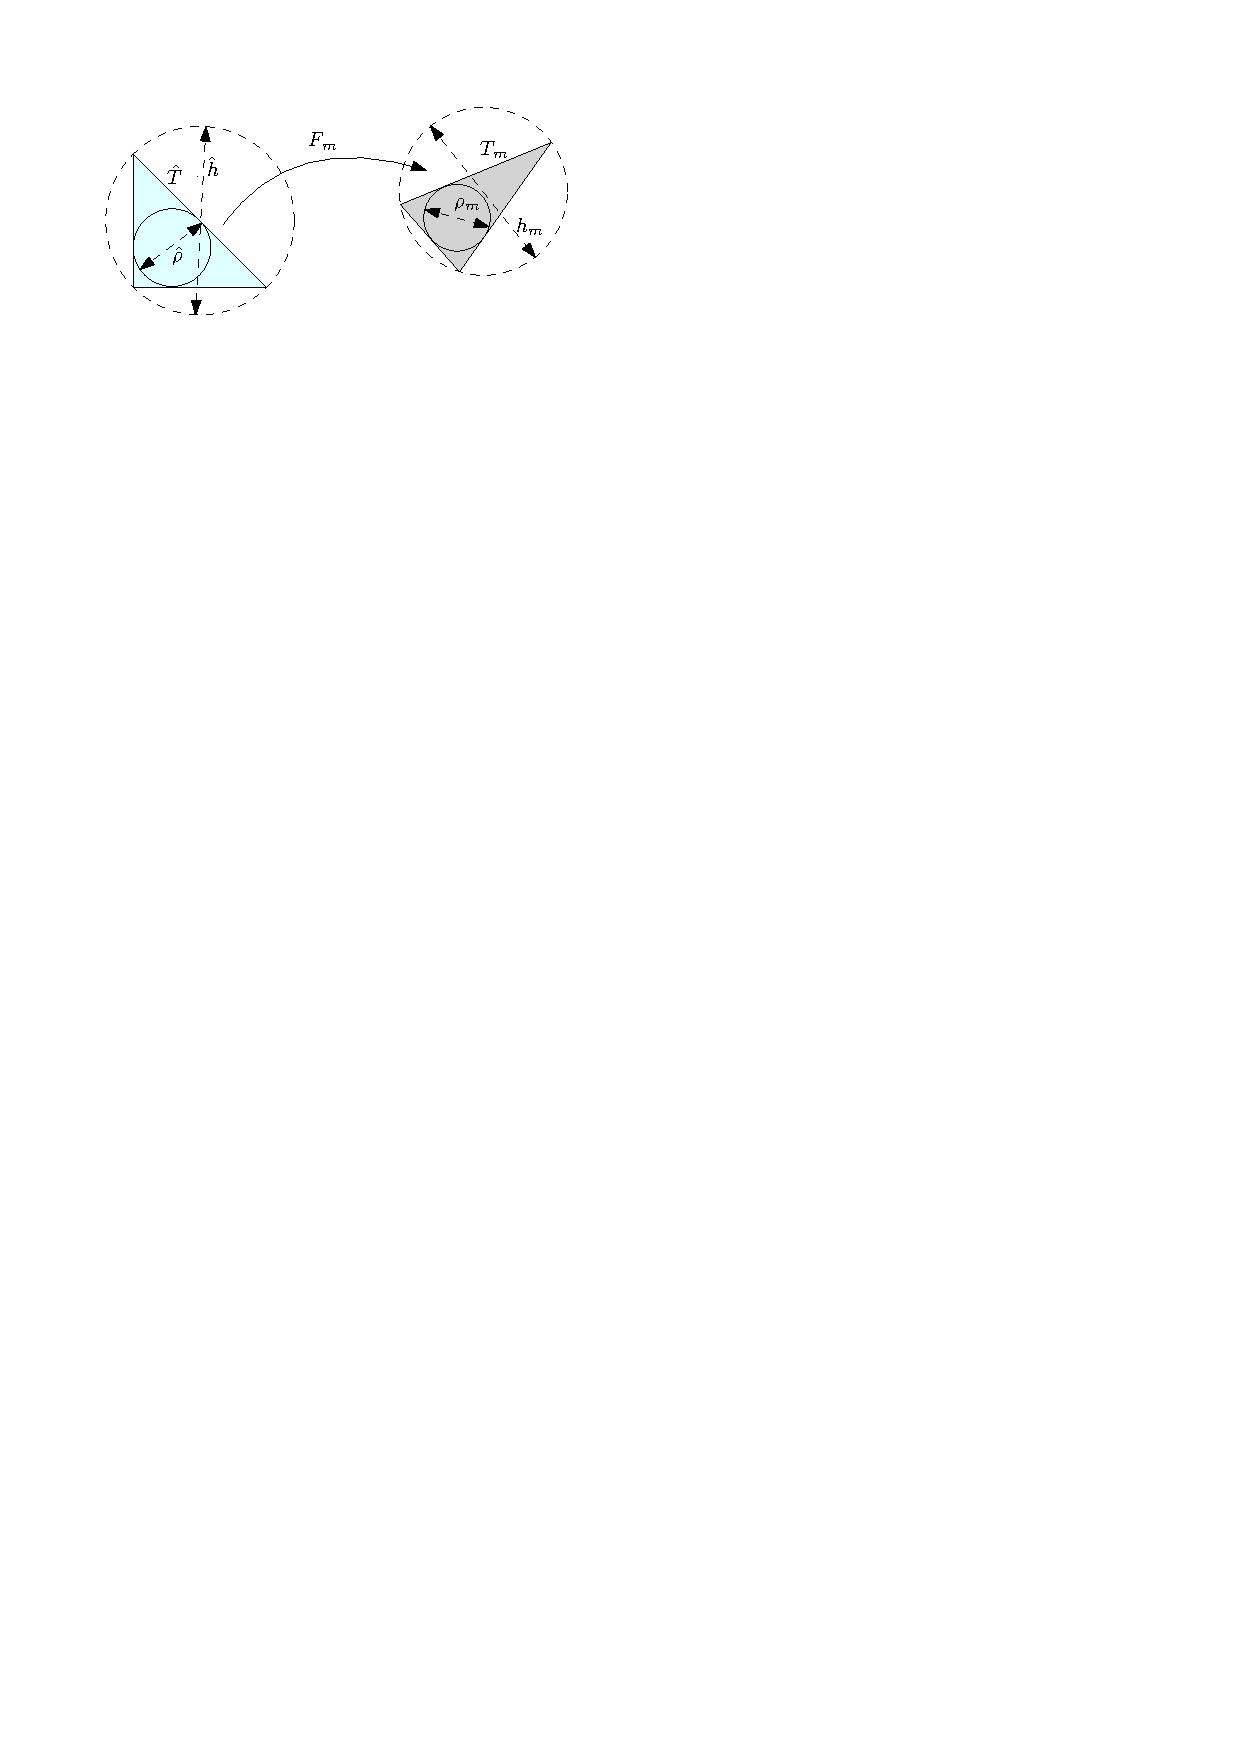
\includegraphics{triangle_scales}
\caption{The scales $\rho_m$ and $h_m$ for a triangle $T_m$, and $\hat \rho$, $\hat h$ for the reference triangle $\hat T$.}
\label{fig:scaling}
\end{figure}


We start with some considerations on the matrix $B$. First, we notice that if $x,y \in T_m$ we have
\[
\abs{x-y} = \abs{B(\hat{x}-\hat{y})} = \abs{B \xi}, \qquad \xi = \hat{x}-\hat{y}.
\]
By the definition of the norm of B, we have that
\[
\norm{B} = \sup_{\abs{\xi} = \hat{\rho}} \frac{\abs{B \xi}}{\abs{\xi}} \le
\sup_{\abs{\xi} = \hat{\rho}} \frac{\abs{x-y}}{\hat{\rho}} \le \frac{h_m}{\hat{\rho}}.
\]
With a similar argument:
\[
\norm{B^{-1}} = \sup_{\abs{\xi} = \rho_m} \frac{\abs{B^{-1} \xi}}{\abs{\xi}} \le \frac{\hat{h}}{\rho_m}
\]
where both $\hat \rho$ and $\hat h$ are constant, and depend only on the choice of the reference triangle $\hat T$.
Also, since $F_m$ is affine, its differential is the matrix $B$ itself. This will come in handy to provide a simple formula for $\hat{D}^\alpha (v \circ F_m)$ when using the chain rule.

Consider a function $v \in \P^l$ on the triangle $T_m$ and let $0\le k \le l$. Then:
\begin{align}
\abs{v \circ F_m}^p_{k,p,\hat{T}} 
&= \sum_{\abs{\alpha} = k} \int_{\hat{T}} \abs{ \hat{D}^\alpha (v \circ F_m)}^p d\hat{T} \\
&= \sum_{\abs{\alpha} = k} \int_{\hat{T}} \abs{ [(D^\alpha v) \circ F_m)] B^{\abs{\alpha}}}^p d\hat{T} \\
&= \sum_{\abs{\alpha} = k} \int_{\hat{T}} \abs{ [(D^\alpha v) \circ F_m)] B^{\abs{\alpha}}}^p J J^{-1} d\hat{T} \\
&= \sum_{\abs{\alpha} = k} \int_{T} \abs{ D^\alpha v B^{\abs{\alpha}}}^p J^{-1} dT \\
&\le \norm{B}^{kp} J^{-1} \sum_{\abs{\alpha} = k} \int_{T} \abs{ D^\alpha v}^p dT
\end{align}
where $J$ is the absolute value of the Jacobian of the transformation $F_m$ (in the present case, $J=\abs{\det B}$). Hence, if we use the inequality we got for $\norm{B}$ we have:
\[
\abs{v \circ F_m}_{k,p,\hat{T}} \le \norm{B}^k J^{-\frac{1}{p}} \abs{v}_{k,p,T}
\le c \Bigl(\frac{h_m}{\hat{\rho}}\Bigr)^k J^{-\frac{1}{p}} \abs{v}_{k,p,T}.
\]

Following the same argument but starting with $\abs{\hat{v} \circ F_m^{-1}}_{k,p,T}$, we obtain:
\[
\abs{v}_{k,p,T} \le \norm{B^{-1}}^k J^{\frac{1}{p}} \abs{v \circ F_m}_{k,p,\hat{T}}
\le c \Bigl(\frac{\rho_m}{\hat{h}}\Bigr)^{-k} J^{\frac{1}{p}} \abs{v \circ F_m}_{k,p,\hat{T}}.
\]

\rev{Polvere: I fixed the previous part. On the next lesson i am going to check in with the teacher what is the correct chain to switch $s$ and $k$. Like this i am not too convinced.}

Combining the two inequalities yields a scaling inequality for any function $v \in \P^l(T)$:
\begin{align}
\abs{v}_{s,p,T} &\le c_1 \rho_m^{-s} J^{\frac{1}{p}} \abs{v \circ F_m}_{s,p,\hat{T}} \\
& \le c_2 \rho_m^{-s} J^{\frac{1}{p}} \abs{v \circ F_m}_{k,p,\hat{T}} \\
& \le c_3 \rho_m^{-s} h_m^k \abs{v}_{k,p,T} \quad \forall 0\le s,k \le l.
\end{align}
The constraint on $s,k$ is there because of the degree of the polynomial (in the formula we have assumed it to be exactly $l$). Notice that we have used the equivalence of norms in finite dimensional spaces (such as $\P^l$) to move from $\abs{v \circ F_m}_{s,p,\hat{T}}$ to $\abs{v \circ F_m}_{k,p,\hat{T}}$.

We would like to make a similar kind of scaling estimate also for functions which are in Sobolev spaces, but are not polynomials. In order to do so, we will need the Bramble-Hilbert lemma.


\section{The Bramble-Hilbert lemma}
From now on we adopt this notation:
\begin{itemize}
\item $a \lesssim b$ means "$\exists c \text{ s.t. } a \le cb$";
\item $a \gtrsim b$ means "$\exists c \text{ s.t. } ca \ge b$";
\item $a \sim b$ means "$a \lesssim b \wedge b \lesssim a$".
\end{itemize}
For example, if two norms $\norm{\cdot}_X$ and $\norm{\cdot}_Y$ are equivalent, the following statements share the same meaning:
\[
\norm{a}_X \sim \norm{a}_Y \iff \exists c,C \text{ s.t. } c\norm{a}_X \le \norm{a}_Y \le C \norm{a}_X.
\]

\begin{lemma}[Bramble-Hilbert]
Let $V$, $W$, $Q$ be Banach spaces and let $\tau \in \L(V,W)$ be an operator such that $Q \subset \ker(\tau)$. Then:
\begin{enumerate}
\item $\norm{\tau(u)}_W \le \norm{\tau}_* \inf_{q \in Q} \norm{u-q}_V \quad \forall u\in V$.
\item Choosing $V=W^{k+1,p}(\Omega)$, $W=W^{s,p}(\Omega)$, $Q=\P^k(\Omega)$, with $\Omega$ open connected (and bounded Lipschitz) and $0\le s \le k$, we get
\[
\norm{\tau(u)}_{s,p,\Omega} \lesssim \norm{\tau}_* \abs{u}_{k+1,p,\Omega} \quad \forall u\in W^{k+1,p}(\Omega).
\]
\end{enumerate}
\end{lemma}
\begin{remark} Meaning...
\rev{say something}
\end{remark}

\begin{proof}
The first inequality is immediate by adding and subtracting $q$ and observing that $\tau(q)=0$:
\[
\tau(u) = \tau(u-q+q) = \tau(u-q) \le \norm{\tau}_* \norm{u-q}.
\]

For the second inequality, the conclusion will follow immediately from the first one (just replace $q$ with $-q$) if we prove that
\[
\abs{u}_{k+1,p,\Omega} \sim \inf_{q \in \P^k} \norm{u+q}_{k+1,p,\Omega}.
\]
This statement is also called in Ciarlet \cite{ciarlet78} the \emph{Deny-Lions lemma}. From now on, we'll omit $\Omega$ for simplicity where its presence is obvious.
\begin{itemize}
\item The inequality $\abs{u}_{k+1,p} \lesssim \inf_{q \in \P^k} \norm{u+q}_{k+1,p}$ is trivial, because every polynomial of degree at most $k$ has zero derivatives of $(k+1)$-th order. Hence
\[
\abs{u}_{k+1,p} = \abs{u+q}_{k+1,p} \le \norm{u+q}_{k+1,p} \quad \forall q \in \P^k.
\]
\item In order to prove that the converse holds, let $\{v_i\}_{i=0}^N$ be a basis for $\P^k$. Then, with the usual notation, $(\P^k)'=\Span\{v^i\}_{i=0}^N$, where the $v^i$-s are such that $v^i(v_j)=\delta_{ij}$. Since $\P^k \subset W^{k+1,p}$, by the Hahn-Banach theorem we can naturally extend these $v^i$-s to be elements of $(W^{k+1,p})'$. Hence we can consider the projection
\begin{align}
\Pi^k:  W^{k+1,p}(\Omega) & \to \P^k(\Omega)\\
u & \mapsto \sum_{i=0}^N v^i(u) v_i.
\end{align}
The key part is proving that
\begin{equation}\label{eqn:deny-lions-exp}
\norm{u}_{k+1,p}^p \sim \abs{u}_{k+1,p}^p + \sum_{i=0}^N \abs{v^i(u)}^p \quad \forall u \in W^{k+1,p}.
\end{equation}
In fact, the $\gtrsim$ inequality follows from bounding the Sobolev seminorm with the corresponding norm and by the simple inequality
\[
\abs{v^i(u)} \le \norm{v^i}_{(W^{k+1,p})'} \norm{u}_{k+1,p}.
\]
The $\lesssim$ inequality, instead, can be proven by contradiction. If it were not true, then for every constant $c$ there would exist $w_c \in W^{k+1,p}$ such that $\norm{w_c}_{k+1,p} = 1$ and
\[
\abs{w_c}_{k+1,p}^p + \sum_{i=0}^N \abs{v^i(w_c)}^p < c \norm{w_c}_{k+1,p}^p = c.
\]
If we choose $c=\frac{1}{j}$, we get a sequence $\{w_j\}$ such that
\begin{equation} \label{eqn:deny-lions-proof}
\abs{w_j}_{k+1,p}^p + \sum_{i=0}^N \abs{v^i(w_j)}^p < \frac{1}{j} \quad \forall j.
\end{equation}
Now, thanks to the compact embedding $W^{k+1,p} \hookrightarrow W^{k,p}$, we have, up to a subsequence, that $w_j \to w$ strongly in $W^{k,p}$ for some $w \in W^{k,p}$.

Actually, the function $w$ belongs to $W^{k+1,p}$. In fact, from~\eqref{eqn:deny-lions-proof} we deduce
\[
\abs{w_j}_{k+1,p}^p < \frac{1}{j} \quad \forall j.
\]
This implies that the sequence $\{w_j\}$ is Cauchy also in $W^{k+1,p}$, because
\[
\norm{w_i-w_j}_{k+1,p}^p = \norm{w_i-w_j}_{k,p}^p + \abs{w_i-w_j}_{k+1,p}^p.
\]
Hence, by uniqueness of the limit, $w \in W^{k+1,p}$. Then, by (strong) continuity of the norm, $\norm{w}_{k+1,p}=1$; also we can pass to the limit the inequality~\eqref{eqn:deny-lions-proof} to get:
\[
\abs{w}_{k+1,p}^p = 0, \quad \sum_{i=0}^N \abs{v^i(w)}^p = 0.
\]
The first equality, since $\Omega$ is an open connected domain, implies that $w \in \P^k(\Omega)$. The second equality implies that $\Pi^k(w)=0$. But for a polynomial in $\P^k$ we have $\Pi^k(w)=w$, hence $w=0$, which is in contradiction with $\norm{w}_{k+1,p}=1$.

We can now conclude, exploiting the inequality~\eqref{eqn:deny-lions-exp}, by noticing that
\begin{align}
\inf_{q \in \P^k} \norm{u+q}_{k+1,p} &\le \norm{u- \Pi^k(u)}_{k+1,p} \\
& \lesssim \abs{u-\Pi^k(u)}_{k+1,p}^p + \sum_{i=0}^N \abs{v^i(u-\Pi^k(u))}^p \\
& = \abs{u}_{k+1,p}^p.
\end{align}
where the last equality holds because the summation term is equal to zero by linearity of the $v^i$-s and the seminorm is simplified due to $\Pi^k(u)$ being a polynomial in $\P^k$.
\end{itemize}
\end{proof}

The Bramble-Hilbert lemma allows us to make error estimates for a finite element method. As in the previous section, consider an affine mapping $F_T: \hat{T} \to T$ and its related quantities $h_T$ and $\rho_T$. If $k$ is the degree of the polynomial approximation of the solution $u$ on $T$, then such an approximation is indeed $\Pi^k(u)$ and the related error is $u-\Pi^k(u)$. Hence we can choose $\tau = Id - \Pi^k$ in the Bramble-Hilbert lemma and repeat the same scaling argument:
\begin{align}
\norm{u- \Pi^k(u)}_{s,p,T} &\lesssim \rho_T^{-s} J^{\frac{1}{p}} \norm{(u- \Pi^k(u)) \circ F_T}_{s,p,\hat{T}} \\
& = \rho_T^{-s} J^{\frac{1}{p}} \norm{u \circ F_T - \Pi^k(u) \circ F_T}_{s,p,\hat{T}} \\
& \lesssim \rho_T^{-s} J^{\frac{1}{p}} \abs{u \circ F_T }_{k+1,p,\hat{T}} \\
& \lesssim h_T^{k+1} \rho_T^{-s} \abs{u}_{k+1,p,T} \quad \forall 0\le s \le k.
\end{align}
This means we can control the Sobolev norm of the error up to order $k$ with the same quantity.
For example: a piecewise linear approximation ($k=1$) allows us to control at most the norm of the gradient of the error. If we also want to control the Laplacian, or the Hessian, then raising the degree of the approximation is mandatory. 

As a follow-up, we can sum over the cells of the triangulation to get a global inequality:
\[
\sum_{T \in \T_h} \norm{u- \Pi^k(u)}_{s,p,T}^p \lesssim
\sum_{T \in \T_h} \bigl( h_T^{k+1} \rho_T^{-s} \abs{u}_{k+1,p,T} \bigr)^p.
\]
If we let
\[
h = \max_{T \in \T_h} h_T, \quad \rho = \min_{T \in \T_h} \rho_T, \quad \Omega = \mathring{\overline{\bigcup_{T \in \T_h} T}}
\]
then we can bound the RHS of the inequality in this way:
\[
\Bigl( \sum_{T \in \T_h} \norm{u- \Pi^k(u)}_{s,p,T}^p \Bigr)^\frac{1}{p} \lesssim
h^{k+1} \rho^{-s} \abs{u}_{k+1,p,\Omega}.
\]
The LHS is called the \emph{broken Sobolev norm} of $u-\Pi^k(u)$, since it is defined element-wise. It is not automatically equal to $\norm{u- \Pi^k(u)}_{s,p,\Omega}$: in order to be, the space $\Omega$ must be \emph{conforming}, i.e. the shape functions must be continuous.
\rev{Specify better what a conforming space is. Here we want that $V_h \subset C^0$, but elsewhere I see $V_h \subset V$, or that $V_h\subset H^s$ means $H^s$-conforming space.}

\begin{remark}
The same inequality can be proven if the triangulation $\T_h$ is made of quadrilaterals. The only difference is that the constants are way better, and this is why meshes with quadrilaterals are used today: they are more difficult to construct, but then the user gets a numerical advantage when approximating the solution.
\end{remark}

Finally, we can couple the estimate from Ceà's lemma~\ref{lemma:cea} with the latter to get the following \emph{a priori} error estimate for finite element methods: provided that $A$ is bounded and coercive and that \emph{we can use} $\norm{\cdot}_{s,p,\Omega}$ as a norm, for a conforming space we have
\begin{align} \label{ineq:cea_scaling}
\norm{u - u_h}_{s,p,\Omega} &\le \frac{\norm{A}}{\alpha} \inf_{v_h \in V_h} \norm{u - v_h}_{s,p,\Omega} \\
& \le \frac{\norm{A}}{\alpha} \norm{u - \Pi^k(u)}_{s,p,\Omega} \\
& \lesssim \frac{\norm{A}}{\alpha} h^{k+1} \rho^{-s} \abs{u}_{k+1,p,\Omega} \quad \forall 0\le s \le k.
\end{align}
The inequality hints at some strategies for error reduction:
\begin{itemize}
\item take $h$ smaller, i.e. \emph{refine the mesh};
\item take $s$ bigger, which implies increasing the polynomial degree.
\end{itemize}
However, there are two very important \emph{caveats}:
\begin{itemize}
\item Since the first line of the inequality relies on Ceà's lemma, we have to check that the space $V$, with $\norm{\cdot}_{s,p,\Omega}$ as a norm, satisfies the hypotheses of the Lax-Milgram lemma. This will likely yield some additional constraint to just requiring $s \in [0,k]$.
\item In order to be able to use the inequality, we need to prove that the solution $u$ is indeed in the space $W^{k+1,p}(\Omega)$, which is not trivial and depends on $A$ and $f$ and on the regularity of the domain $\Omega$. This is what the theory of regularity for PDEs attempts to do. In particular, in the following section we will mention the concept of $r$-regularity.
\end{itemize}

%%%%%
% Lecture of 27 of March
%%%%%


\section{\texorpdfstring{$H^k$}{Hk} error estimates, Nitsche's lemma}
Consider a triangulation $\T_h$ and recall the quantities $h$ and $\rho$ we defined in the previous section:
\[
h := \max_{T \in \T_h} h_T, \quad \rho := \min_{T \in \T_h} \rho_T.
\]
We say that the mesh is \emph{quasi-uniform} if
\[
\exists \sigma > 0 \text{ s.t. } \rho_T \ge \sigma h_T  \quad \forall T\in \T_h.
\]
For such a mesh, the inequality~\eqref{ineq:cea_scaling} becomes:
\begin{equation} \label{ineq:cea_scaling2}
\norm{u - u_h}_{s,p,\Omega}
\lesssim \frac{\norm{A}}{\alpha} h^{k+1-s} \abs{u}_{k+1,p,\Omega} \quad \forall 0\le s \le k.
\end{equation}
From now on we consider $p=2$ and use the notation $\norm{u}_k$ to mean $\norm{u}_{k,2,\Omega}$.
\begin{definition}
Let $V \subset H^k$ and $A \in \L(V,V')$. We say that $A$ is $r$-\emph{regular} if there exists an interval $[s_{min}, s_{max}]$ such that $\forall g \in H^s$, with $s \in [s_{min}, s_{max}]$, the problem $Au=f$ admits a unique solution $u$ which satisfies
\[
\norm{u}_{s+r} \lesssim \norm{f}_s.
\]
\end{definition}
\rev{Check if on the LHS there is norm or seminorm of $u$.}
The inequality~\eqref{ineq:cea_scaling2}, combined with the assumption of $r$-regularity, becomes
\begin{equation}\label{ineq:cea_scaling3}
\norm{u-u_h}_k \lesssim h^{s+r-k} \abs{u}_{s+r} \lesssim h^{s+r-k} \norm{f}_s \quad \forall 0\le k \le s+r-1.
\end{equation}
This is finally the error estimate we were looking for. However, as said before, we may not be allowed to use all the values for $k$ in the range above, as the following example will show.
\begin{example}
The Poisson problem on a Lipschitz, convex domain is $2$-regular, with $s \le 0$. Hence, the inequality~\eqref{ineq:cea_scaling3} becomes
\[
\norm{u-u_h}_k \lesssim h^{s+2-k} \norm{f}_s \quad \forall 0\le k \le s+1.
\]
In particular, if $k=1$, we get
\[
\norm{u-u_h}_1 \lesssim h^{s+1} \norm{f}_s.
\]
This means that, for instance, if $f \in L^2$, i.e. $s=0$, the order of convergence in the $H^1$ norm is $1$. If $\Omega$ is better than Lipschitz, then the range for $s$ becomes better, hence we gain a better convergence of the numerical approximation (provided that $f$ is more regular).
Unfortunately, we cannot use the $L^2$ norm in Ceà's lemma, and this means that we cannot get an estimate in the $L^2$ norm.
\end{example}

With some bit of additional work, we can produce error estimates on weaker norms, such as the $L^2$ one, from the estimates on stronger norms.
\begin{lemma}[Nitsche] \label{lemma:nitsche}
Let $A \in \L(V,V')$ an operator as in the hypotheses of Lax-Milgram's lemma. Assume that $V$ is a subspace of some Hilbert space $H$, with the following properties:
\begin{romanlist}
\item $\norm{u}_H \lesssim \norm{u}_V$ $\quad \forall u \in V$ \quad (i.e., the embedding $V \hookrightarrow H$ is continuous);
\item $V = \overline{H}^{\norm{\cdot}_V}$.
\end{romanlist}
Then the following inequality holds:
\begin{equation}\label{eqn:nitsche_lemma}
\norm{u-u_h}_H \lesssim \sup_{g \in H} \Bigl( \frac{1}{\norm{g}_H} \inf_{\phi_h \in V_h} \norm{\phi_g - \phi_h}_V \Bigr) \norm{u-u_h}_V .
\end{equation}
\end{lemma}

\begin{remark}
With the hypotheses above, if $f \in H$, by the Hahn-Banach theorem $f$ can be extended to a functional $\tilde{f} \in V'$, i.e.
\[
\langle \tilde{f}, v \rangle_V = (f, v)_H \quad \forall v \in V.
\]
\rev{Is Hahn-Banach really necessary? We are in a Hilbert space setting.}
Now consider the usual problem in operator form $A u = \tilde{f}$, i.e.
\begin{equation}
\langle Au,v \rangle = \langle \tilde{f},v \rangle = (f, v)_H \quad \forall v\in V.
\end{equation}
By the Lax-Milgram lemma, we know that this problem has a unique solution $u \in V$.

With the same philosophy, let $g \in H$ and consider the \emph{dual problem} $A^T \phi = g$, i.e.
\begin{equation}
\langle Av,\phi \rangle = \langle \tilde{g},v \rangle = (g, v)_H \quad \forall v\in V.
\end{equation}
Since also $A^T$ satisfies the hypotheses of the Lax-Milgram lemma, the adjoint problem admits itself a unique solution $\phi_g \in V$.
\end{remark}

\begin{proof}
We start observing that
\begin{equation}\label{eqn:nitsche_norm}
\norm{u-u_h}_H = \sup_{g \in H} \frac{(g, u-u_h)_H}{\norm{g}_H}.
\end{equation}
This is true because $H$ is a Hilbert space, hence $H \cong H'$.

Given $g \in H$, we know from the last remark that the dual problem $A^T \phi = g$ admits a unique solution $\phi_g \in V$. If we set $v = u-u_h$, we get:
\[
\langle A (u-u_h),\phi_g \rangle = (g, u-u_h)_H.
\]
Now we take advantage of the Galerkin orthogonality, i.e. $\langle A (u-u_h), \phi_h \rangle = 0$ $\forall \phi_h \in V_h$:
\[
(g, u-u_h)_H = \langle A (u-u_h),\phi_g - \phi_h \rangle \quad \forall \phi_h \in V_h.
\]
Now we use the continuity of $A$ on~\eqref{eqn:nitsche_norm} to produce the desired estimate:
\begin{align}
\norm{u-u_h}_H &= \sup_{g \in H} \frac{(g, u-u_h)_H}{\norm{g}_H} \\
& = \sup_{g \in H} \frac{\langle A (u-u_h),\phi_g - \phi_h \rangle}{\norm{g}_H} \\
& \le \norm{A} \sup_{g \in H} \Bigl( \frac{1}{\norm{g}_H} \inf_{\phi_h \in V_h} \norm{\phi_g - \phi_h}_V \Bigr)
\norm{u-u_h}_V .
\end{align}
\end{proof}

In practice, we want to use this lemma with $V \subset H^k$ and $H \subset H^s$, with $0\le s < k$, or at least we want that $\norm{\cdot}_V \sim \norm{\cdot}_k$ and $\norm{\cdot}_H \sim \norm{\cdot}_s$. For instance, think as $V=H^1$, $H=L^2$.
\rev{Fix inconsistencies between $\Pi^k$ and $I_h$.}
In order to find a relation between $\norm{\phi_g - \phi_h}_k$ and $\norm{g}_s$, we use the Bramble-Hilbert lemma and the scaling argument, plus the $r$-regularity, but for $A^T$:
\begin{align}
\inf_{\phi_h \in V_h} \norm{\phi_g - \phi_h}_k &\lesssim \norm{\phi_g - I_h(\phi_g)}_k  \\
&\lesssim h^{s+r-k} \abs{\phi_g}_{s+r}  \\
&\lesssim h^{s+r-k} \norm{g}_s.
\end{align}
\emph{Careful}, though: this is true as soon as $s+r-k \ge 0$, i.e. $s \ge k-r$. Hence, Nitsche's lemma extends the range of available Sobolev norms for the error estimate according to the regularity of the operator. Plugging the result into the inequality~\eqref{eqn:nitsche_lemma} of the Nitsche lemma, we get:
\[
\norm{u-u_h}_s \lesssim h^{s+r-k} \norm{u-u_h}_k \quad \text{if $s \ge k-r$}.
\]

\begin{example}
Back to the Poisson problem on a Lipschitz, convex domain: we have now an estimate for the $L^2$ norm of the error. We pick $s = 0$ and $k=1$ to get
\[
\norm{u-u_h}_0 \lesssim h \norm{u-u_h}_1.
\]
We had proven before that
\[
\norm{u-u_h}_1 \lesssim h^{t+1} \norm{f}_t
\]
for $t$ in an appropriate range, depending on the regularity of $\Omega$. Hence:
\[
\norm{u-u_h}_0 \lesssim h^{t+2} \norm{f}_t.
\]
For instance, if $t=0$, we have convergence of order $1$ in $H^1$, of order $2$ in $L^2$. This behavior corresponds to what we see numerically: the convergence in a lower order Sobolev norm is better than a higher order one.
\end{example}


\section{Inverse estimates}
Suppose that $V_h \subset H^k$ and let $v \in V_h$. In the previous sections we have proved that, for quasi-uniform meshes, on each triangle $T$ the following inequality holds:
\[
\abs{v}_{s,p,T} \lesssim h^{k-s} \abs{v}_{k,p,T} \quad \forall 0 \le s \le k.
\]
With the same scaling argument, we can also prove that, if $h<1$, then
\[
\abs{v}_{s,p,T} \lesssim h^{k-s} \abs{v}_{k,p,T} \quad \forall 0 \le k \le s.
\]
Of course, in either case, $k$, $s$ must be chosen smaller or equal to the degree of $v$. The proof relies once more on the fact that all norms in finite dimensional spaces are equivalent.

\emph{Nota bene}: this is true only for finite element functions!
\rev{Expand more on the proof.}

\section{Trace operators}\label{sec:trace_operators}
In order to deal with the trace of a Sobolev function, it is necessary to give a meaning to the space $W^{s,p}(\Omega)$ for $s\in \R$. Here we will only present the fundamental concepts. For extensive reference, see~\cite{fract_sob}. For a Lipschitz domain $\Omega \subset \R^d$ we can also define the space $W^{s,p}(\Omega)$ in a different way. We let $\lambda \in (0,1)$ such that $s = m+\lambda$ for an integer $m$ and consider the following norm:
\[
\norm{u}_{s,p}^p := \norm{u}_{m,p}^p + \sum_{\abs{\alpha}=m} \abs{D^\alpha u}^p_{\lambda,p}
\]
where $\abs{u}_{\lambda,p}$ is called in literature the \emph{Gagliardo seminorm} of $u$:
\[
\abs{u}^p_{\lambda,p} := \int_{\Omega} \int_{\Omega} \frac{\abs{u(x)-u(y)}^p}{\abs{x-y}^{d+\lambda p}} \diff x \,dy.
\]
Then we define
\[
W^{s,p}(\Omega) := \Set{u \in W^{m,p}(\Omega) : \norm{u}_{s,p}^p < +\infty}.
\]
As in the case $s \in \N$, we also have that $W^{s,p}_0(\Omega) = \overline{C^\infty_0(\Omega)}^{\norm{\cdot}_{s,p}}$. One can prove that the spaces we have constructed are Banach spaces. Moreover, if we restrict to the case $p=2$, they turn out to be Hilbert spaces.

For the case $p=2$, if $\Omega = \R^d$, there is an equivalent definition of the space $H^s(\R^d)$ via the Fourier transform $\F$:
\[
\bigl(\F u\bigr)(\xi) := \Bigl(\frac{1}{2\pi} \Bigr)^{d/2} \int_{\R^d} e^{-i \xi \cdot x} u(x) \diff x.
\]
If we consider the Schwartz space $\mathcal{S}$ of rapidly decaying $C^\infty$ functions in $\R^d$, then $H^s(\R^d)$ can be defined as a subspace of tempered distributions:
\[
H^s(\R^d) := \Set{u \in \mathcal{S}' : \norm{u}_s < +\infty}
\]
where the norm is
\[
\norm{u}_s := \norm{\abs{(1+\abs{\cdot}^2)}^{\frac{s}{2}} \F u(\cdot)}_{L^2(\R^d)}.
\]
In particular, as before we have $H^s_0(\R^d) = \overline{C^\infty_0(\R^d)}^{\norm{\cdot}_s}$.
Without going into detail, the main reason of the equivalence ot the two formulation is Plancherel's formula for the Fourier transform, which is specific for $p=2$. There is no equivalence for different values of $p$.

Now let $\Omega \subset \R^d$ be a Lipschitz domain and $\Gamma$ its boundary. If $u \in H^s(\Omega) \not\subset C^0(\Omega)$, then $\restr{u}{\Gamma}$ makes no sense pointwise. For example, $H^1$ functions are not continuous for $d \ge 2$. In order to give some sense to the expression $\restr{u}{\Gamma}$, we introduce the \emph{trace operator}:
\begin{theorem}[Trace theorem]
Let $\Omega \subset \R^d$ be a Lipschitz domain and $s \in (\frac{1}{2}, 1]$. Then there exists a unique linear bounded mapping
\[
\gamma: H^s(\Omega) \to H^{s-\frac{1}{2}}(\Gamma)
\]
such that:
\begin{enumerate}
\item For every $u \in C^0(\overline{\Omega})$, $\gamma u = \restr{u}{\Gamma}$.
\item For every $v \in H^s(\Omega)$, $\norm{\gamma v}_{s-\frac{1}{2},\Gamma} \lesssim \norm{v}_{s,\Omega}$.
\item $\gamma$ admits a bounded right inverse
\[
E: H^{s-\frac{1}{2}}(\Gamma) \to H^s(\Omega)
\]
i.e. $\forall g\in H^{s-\frac{1}{2}}(\Gamma)$ we have $\norm{E g}_{s,\Omega} \lesssim \norm{g}_{s-\frac{1}{2},\Gamma}$ and $\gamma E g = g$.
\end{enumerate}
In particular, $\ker(\gamma) = H^s_0(\Omega) = \Set{u \in H^s(\Omega) : \gamma u = 0}$.
\end{theorem}

Trace is a fundamental concept when dealing with boundary conditions. Consider as a motivating example the Poisson problem on $\Omega$ with both Dirichlet and Neumann boundary conditions:
\[
\begin{cases} 
-\Delta u = f \qquad &\text{in $\Omega$} \\
u =  g_D \qquad &\text{on $\Gamma_D$} \\
\frac{\partial u}{\partial n} =  g_N \qquad &\text{on $\Gamma_N$}
\end{cases}
\]
where $\Gamma_D$ and $\Gamma_N$ are contained in $\Gamma$. If $u \in H^1$, then its restriction to $\Gamma$ is not well defined. In order to handle Dirichlet boundary conditions, we can resort to the trace operator (with restricted codomain) $\gamma_{_{\Gamma_D}}: H^1(\Omega) \to H^{\frac{1}{2}}(\Gamma_D)$ and require that $\gamma_{_{\Gamma_D}} u = g_D$. However, this trick fails with $\frac{\partial u}{\partial n} \in L^2$, because even its trace makes no sense! We solve this problem incorporating the Neumann boundary condition into the weak form.
To make things clearer: we let
\begin{align}
V_{0,\Gamma_D} &:= \Set{u \in H^1(\Omega) : \gamma_{_{\Gamma_D}}=0}, \\
V_{g_D,\Gamma_D} &:= V_{0,\Gamma_D} + u_D, \quad \text{where } \gamma_{_{\Gamma_D}} u_D = g_D.
\end{align}
The new weak form is: find $u \in V_{g_D,\Gamma_D}$ such that
\[
(\nabla u, \nabla v) = \langle f, v \rangle + \int_{\Gamma_N} g_N v \quad \forall v \in V_{0,\Gamma_D}.
\]
In particular, the minimal regularity we need to require for $f$, $g_D$, $g_N$ is:
\[
f \in \bigl(H^1(\Omega)\bigr)', \quad g_D \in H^\frac{1}{2}(\Gamma_D), \quad g_N \in \bigl(H^\frac{1}{2}(\Gamma_N)\bigr)'.
\]

To conclude this section, let's make a concrete example of coupling the inverse and trace inequalities we have seen so far. If $s>\frac{1}{2}$ and $u \in \P^k(T) \subset H^s(T)$, we have:
\[
\norm{u}_{s-\frac{1}{2},\partial T} \lesssim \norm{u}_{s,T} \lesssim h^{r-s} \norm{u}_{r,T}.
\]
In particular...
\rev{Understand and complete the example from the notes.}

\rev{something missing from start of following lecture}
